% !TEX root = ../main.tex

\section{Timing}
\label{sec:results-timing}

For the recognition time, the oscilloscope recorded the tip switch and the ring of one jack, triggered by the plug lifting the tip switch; every change of the drive pattern shows on the ring, so the phases of the jack monitor can be read off. With rails measured less than \qty{30}{\second} before, a potentiometer pedal was followed 65 to \qty{95}{\milli\second} after insertion in five runs (\cref{fig:plug-in-fresh}): up to \qty{50}{\milli\second} until the next plug check and 44 to \qty{48}{\milli\second} of identification. Otherwise, the rails are measured first, which takes \qty{214}{\milli\second} and gives about \qty{300}{\milli\second} in total (\cref{fig:plug-in-refresh}). Unplugging was noticed within 2 to \qty{27}{\milli\second}, and the jack reported empty after 260 to \qty{391}{\milli\second} in three runs, again mostly because of the rail measurement (\cref{fig:unplug}). \Cref{tab:plug-in} lists all runs, and \cref{fig:plug-unplug} shows the two remaining captures.

\begin{figure}[tb]
  \centering
  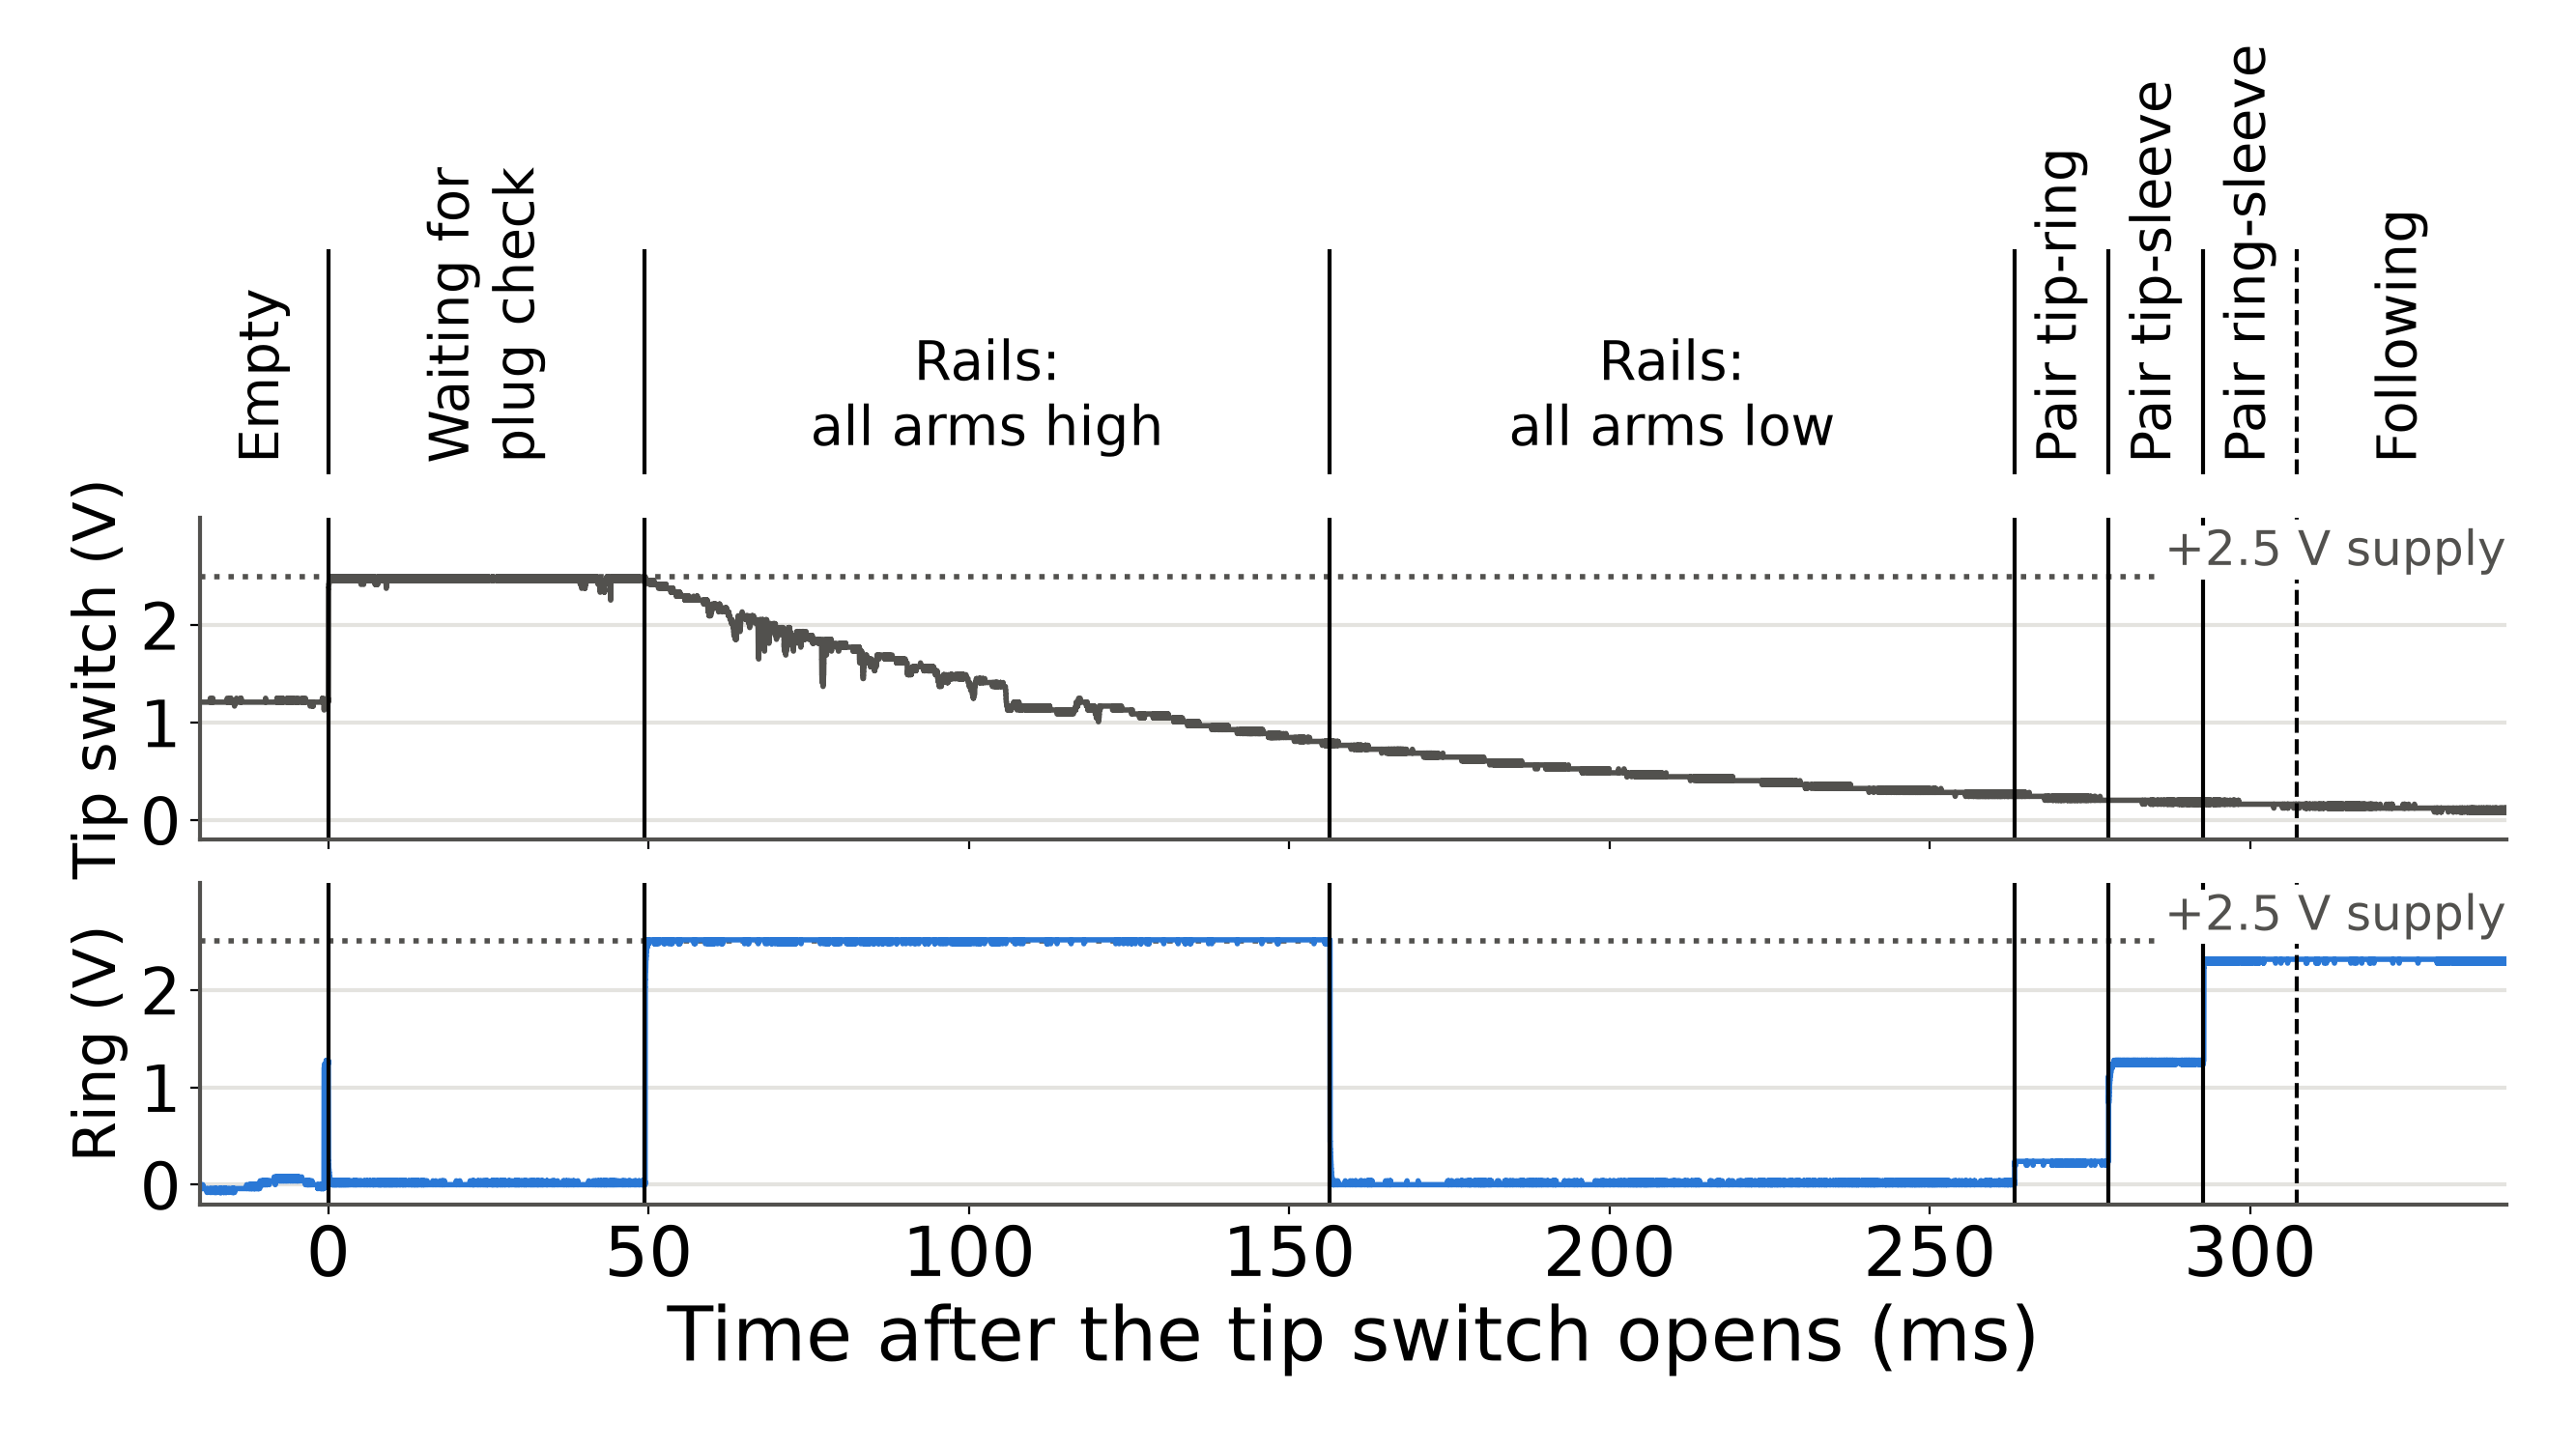
\includegraphics[width=0.6\linewidth]{05-results/figures/plug-in-rail-refresh}
  \titledcaption{Plug-In with Rail Measurement}{Tip switch (top) and ring (bottom) of one jack while a potentiometer pedal is plugged in with rails older than \qty{30}{\second}, 10X probes, triggered when the tip switch opens at \qty{0}{\milli\second}. Vertical lines are latch edges of the shift register; the dashed line, the start of following, is inferred from the length of one pair.}
  \label{fig:plug-in-refresh}
\end{figure}

An earlier capture of a power-up with the EV-30 plugged in contains a floating ring charging through the pedal. The fitted time constant was \qty{190.6}{\micro\second}, against $(R_\mathrm{net} + R_\mathrm{f})\,C_\mathrm{f} = \qty{194}{\micro\second}$ from \cref{eq:settling}, and \qty{3.2}{\milli\volt} remained after the minimum wait of \qty{1}{\milli\second}. A series with known resistors up to \qty{220}{\kilo\ohm}, which would test the settling model at its limit, was left out in favor of the other measurements.

The firmware logged 188 to 189 updates per second for one pedal on its ADC, against 2.6 for the first firmware, and about the expected 95 per jack for two pedals on one ADC. All four jacks were run at once with two expression pedals, a footswitch and an open cable. The complete end-to-end latency, from a pedal movement to the audible result, was too difficult to measure directly and is estimated instead: Within the adapter, a movement waits at most one reading interval, \qty{5.3}{\milli\second} for one pedal on its ADC or \qty{10.5}{\milli\second} for two pedals on one ADC, and half of that on average; the USB transfer adds at most the next frame of \qty{1}{\milli\second}. The part of the latency this project can influence is therefore set almost entirely by the ADC readings, not by the USB stack. The host adds its own USB stack and the audio buffer of the music software, which lie outside the adapter, \qty{5.3}{\milli\second} alone for 256 samples at \qty{48}{\kilo\hertz}. With one pedal per ADC, the adapter thus adds at most about as much as this buffer and stays well below the bound of \qty{10}{\milli\second} given in \cref{sec:firmware}; with two pedals on one ADC, its worst case of \qty{11.5}{\milli\second} reaches this bound, while the average of about \qty{6}{\milli\second} stays below it, and both configurations meet the target of 50 to 100 updates per second and jack.
